%%=====================================================================
%% SBESC 2026 -- XVI Symposium on Computing Systems Engineering
%% Main track: IEEE two-column conference template (max 6 pages).
%% English full papers are published in IEEE Xplore (CPS).
%% Submission: JEMS3 -> https://jems3.sbc.org.br/events/628  (deadline: 2026-07-10)
%%
%% HOW TO BUILD:
%%   Recommended: upload this .tex to Overleaf, set compiler to pdfLaTeX,
%%   and download the PDF. No external image files are required
%%   (the architecture figure is drawn with TikZ).
%%
%% BEFORE SUBMITTING (fill in / double-check):
%%   - author e-mails (the second one is a placeholder)
%%   - confirm the 6-page limit is respected in the final PDF
%%=====================================================================
\documentclass[conference]{IEEEtran}
\IEEEoverridecommandlockouts

\usepackage{cite}
\usepackage{amsmath,amssymb,amsfonts}
\usepackage{graphicx}
\usepackage{booktabs}
\usepackage{array}
\usepackage{tikz}
\usetikzlibrary{positioning,arrows.meta}
\usepackage[hidelinks]{hyperref}
\usepackage{url}
\def\BibTeX{{\rm B\kern-.05em{\sc i\kern-.025em b}\kern-.08em T\kern-.1667em\lower.7ex\hbox{E}\kern-.125emX}}

\begin{document}

\title{Autonomous Contextual Authentication for Web\\ Applications Combining an AI Ensemble and\\ Permissioned Blockchain Auditing}

\author{\IEEEauthorblockN{Jo\~ao Guedes de Brito}
\IEEEauthorblockA{\textit{Graduate Program in Systems and Products Engineering (PPGESP)}\\
\textit{Instituto Federal da Bahia (IFBA)}\\
Salvador, Bahia, Brazil \\
joaoguedesdebrito@gmail.com}
\and
\IEEEauthorblockN{Cleber Jorge Lira de Santana}
\IEEEauthorblockA{\textit{Graduate Program in Systems and Products Engineering (PPGESP)}\\
\textit{Instituto Federal da Bahia (IFBA)}\\
Salvador, Bahia, Brazil \\
cleber.santana@ifba.edu.br}
}

\maketitle

\begin{abstract}
Traditional authentication mechanisms based on static passwords or
fixed multi-factor authentication (MFA) remain widely deployed, yet
they ignore the behavioral and environmental context of each access
attempt and are increasingly exploited by credential stuffing,
phishing, and account-takeover attacks. This paper presents an
autonomous contextual authentication system for web applications that
combines a machine-learning ensemble with permissioned-blockchain
auditing. Each login is described by fourteen contextual and
behavioral features, which are scored by an ensemble of Isolation
Forest, Random Forest, and a multilayer neural network; the resulting
risk score drives a three-band adaptive decision (grant, step-up to
MFA, or block). Every decision is recorded immutably on a Hyperledger
Fabric ledger, yielding a verifiable, non-repudiable audit trail whose
necessity over signed logs and append-only databases is explicitly
justified. In a controlled evaluation on a synthetic dataset of about
50{,}000 login records (95\% legitimate, 5\% suspicious), the ensemble
reached 98.1\% accuracy, 80.6\% F1-score, and a 0.99 ROC-AUC on a
held-out test set, with a 1.0\% false-positive rate and an inference
latency of roughly 18.6\,ms per request. These results are preliminary
and rely on synthetic data; they characterize the technical
feasibility of the approach rather than a field study, and are to be
confirmed with real data.
\end{abstract}

\begin{IEEEkeywords}
contextual authentication, risk-based authentication, machine
learning, ensemble, anomaly detection, blockchain, audit trail,
information security.
\end{IEEEkeywords}

\section{Introduction}
Authentication is the first line of defense of web applications.
Historically it has relied on a knowledge factor---the
password---whose weaknesses are well documented: passwords are reused
across services, leaked at scale, and exploited through brute force,
credential stuffing, and phishing~\cite{nist80063b,verizon2024}.
Multi-factor authentication (MFA) mitigates part of this exposure by
combining knowledge, possession, and inherence factors, but static MFA
still falls to social engineering, SIM swapping, and real-time code
interception, while adding friction to the user
experience~\cite{nist80063b}.

To address these limitations, the NIST digital identity
guidelines and the Zero Trust model recommend \emph{adaptive}
mechanisms, in which the level of verification required is proportional
to the estimated risk of each attempt~\cite{nist80063b,rose2020}. This
shifts authentication from a binary, static decision toward a
continuous, context-sensitive assessment---an approach known in the
literature as risk-based authentication (RBA). Empirical studies of
production services show, however, that deployed RBA is dominated by a
single signal (typically the IP address) and by hand-tuned
heuristics~\cite{wiefling2019,wiefling2023}. In parallel, when access
decisions are delegated to autonomous models, they must be
\emph{auditable} by third parties (e.g., for regulatory compliance), a
requirement that decision logs held by a single operator do not fully
satisfy.

This paper proposes an autonomous contextual authentication system
that unifies, in a single flow, an adaptive machine-learning (ML)
decision and its immutable audit. The main contributions are:
\begin{itemize}
  \item an end-to-end architecture that fuses fourteen contextual and
        behavioral features into a single risk score computed by an
        ensemble of Isolation Forest, Random Forest, and a neural
        network, driving a three-band adaptive decision;
  \item a permissioned-blockchain audit layer coupled to the decision,
        with an explicit justification of \emph{why} a blockchain is
        needed over signed logs or append-only databases; and
  \item a reproducible evaluation methodology, with baselines and a
        preliminary feasibility study on synthetic data.
\end{itemize}

The remainder of the paper is organized as follows. Section~\ref{sec:related}
reviews related work. Section~\ref{sec:arch} describes the proposed
architecture, Section~\ref{sec:ai} the AI decision engine, and
Section~\ref{sec:bc} the blockchain audit layer.
Section~\ref{sec:method} presents the evaluation methodology and
Section~\ref{sec:results} the results. Section~\ref{sec:conclusion}
concludes.

\section{Related Work}
\label{sec:related}
\textbf{Behavioral biometrics.} Continuous authentication from
interaction patterns is well established. TypeNet~\cite{acien2022} and
TypeFormer~\cite{stragapede2024} identify users from keystroke dynamics
with low error rates, and Touchalytics~\cite{frank2013} shows that
touchscreen patterns discriminate users on mobile devices. These works
confirm the discriminative power of user behavior but focus on a
single biometric modality and do not address immutable auditing of the
decisions.

\textbf{Risk-based authentication.} Wiefling \emph{et
al.}~\cite{wiefling2019} conducted the first large-scale empirical
study of RBA in the wild, and later work~\cite{wiefling2023} showed
that risk factors must be carefully tuned per service. Our proposal
follows this line but replaces fixed heuristics with an ML ensemble and
adds a non-repudiation layer.

\textbf{Anomaly detection.} Isolation Forest~\cite{liu2008} is a
reference for unsupervised outlier detection in high-dimensional
spaces, and supervised and deep models~\cite{goodfellow2016} complement
it when labels are available; Killourhy and Maxion~\cite{killourhy2009}
established a methodological benchmark for keystroke anomaly detection.
We combine both natures---unsupervised and supervised---in an ensemble.

\textbf{Blockchain for auditing.} Although blockchain-based log
auditing has been investigated, most approaches treat event recording
as \emph{decoupled} from the decision mechanism. The distinguishing
feature of this work is to integrate, in a single flow, the adaptive
AI decision and its immutable record on a permissioned ledger.
Table~\ref{tab:related} summarizes representative work: no single line
of research simultaneously provides (i)~fusion of multiple contextual
and behavioral signals, (ii)~an adaptive ensemble decision, and
(iii)~audit immutability coupled to the decision.

\begin{table}[t]
\caption{Positioning Against Representative Related Work}
\label{tab:related}
\centering
\renewcommand{\arraystretch}{1.2}
\begin{tabular}{@{}p{1.55cm}p{2.0cm}p{3.0cm}@{}}
\toprule
\textbf{Work} & \textbf{Technique} & \textbf{Main limitation} \\
\midrule
TypeNet~\cite{acien2022} & Recurrent neural net & Single modality; no decision audit \\
Touchalytics~\cite{frank2013} & SVM / $k$-NN & Restricted to touchscreens \\
RBA~\cite{wiefling2019} & Heuristics/statistics & Fixed rules; no adaptive AI \\
Isolation Forest~\cite{liu2008} & Unsupervised & Isolated signal; does not decide access \\
\textbf{This work} & Ensemble (IF+RF+DL) + blockchain & Integrates the three axes in one flow \\
\bottomrule
\end{tabular}
\end{table}

\section{Proposed Architecture}
\label{sec:arch}
The architecture articulates microservices, federated identity
management, AI-based risk analysis, and immutable blockchain recording,
following the principles of security by design and continuous
verification of Zero Trust~\cite{rose2020,nist80053r5}. Rather than a
binary decision at login time, the model adopts a continuous,
risk-oriented perspective. It is organized in five integrated layers
(Fig.~\ref{fig:arch}):

\begin{enumerate}
  \item \textbf{Modular Application.} Independent services (Spring
        Boot) and an Angular front end exposing authenticated REST APIs.
  \item \textbf{Identity and Access.} Federated authentication through
        Keycloak (OAuth2 / OpenID Connect), JWT issuance, and MFA
        support.
  \item \textbf{Contextual Intelligence.} Extraction of the fourteen
        behavioral features and computation of the risk score by the
        ensemble.
  \item \textbf{Adaptive Decision.} Application of the risk thresholds,
        resulting in \emph{grant}, \emph{step-up to MFA}, or
        \emph{block}.
  \item \textbf{Immutable Registry and Audit.} Persistence of each
        decision on a permissioned blockchain, ensuring traceability
        and non-repudiation.
\end{enumerate}

The operational flow is a chained decision pipeline: a login attempt
triggers extraction of the contextual features; the AI engine computes
the risk score; the decision thresholds are applied; the outcome is
recorded on the blockchain; and the system grants access, requires MFA,
or blocks the attempt. The separation into layers allows each
responsibility to evolve independently and specific security policies
to be enforced at each level.

\begin{figure}[t]
\centering
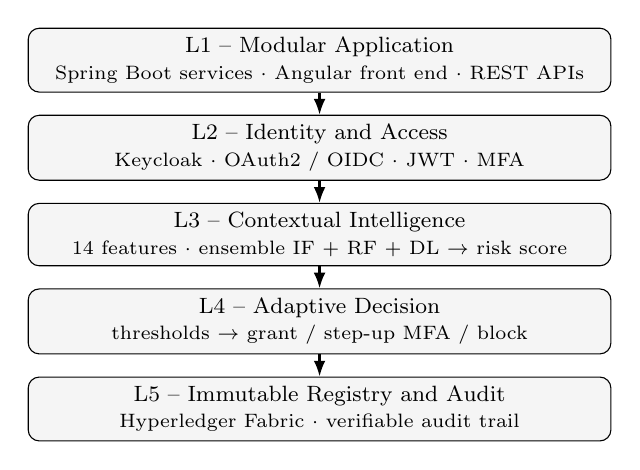
\begin{tikzpicture}[
  layer/.style={draw, rounded corners, minimum width=7.4cm,
    minimum height=0.72cm, align=center, font=\footnotesize, fill=gray!8},
  arr/.style={-{Latex[length=2mm]}, thick}
]
\node[layer] (l1) {L1 -- Modular Application \\ \scriptsize Spring Boot services $\cdot$ Angular front end $\cdot$ REST APIs};
\node[layer, below=0.28cm of l1] (l2) {L2 -- Identity and Access \\ \scriptsize Keycloak $\cdot$ OAuth2 / OIDC $\cdot$ JWT $\cdot$ MFA};
\node[layer, below=0.28cm of l2] (l3) {L3 -- Contextual Intelligence \\ \scriptsize 14 features $\cdot$ ensemble IF + RF + DL $\rightarrow$ risk score};
\node[layer, below=0.28cm of l3] (l4) {L4 -- Adaptive Decision \\ \scriptsize thresholds $\rightarrow$ grant / step-up MFA / block};
\node[layer, below=0.28cm of l4] (l5) {L5 -- Immutable Registry and Audit \\ \scriptsize Hyperledger Fabric $\cdot$ verifiable audit trail};
\draw[arr] (l1) -- (l2);
\draw[arr] (l2) -- (l3);
\draw[arr] (l3) -- (l4);
\draw[arr] (l4) -- (l5);
\end{tikzpicture}
\caption{Five-layer architecture of the proposed system.}
\label{fig:arch}
\end{figure}

\section{AI Decision Engine}
\label{sec:ai}
\textbf{Ensemble.} The risk engine combines three complementary
learners. \emph{Isolation Forest}~\cite{liu2008} acts as the first
level of analysis, isolating outliers in the multidimensional feature
space with few random partitions; it contributes 40\% of the final
weight. \emph{Random Forest} contributes 30\%, capturing non-linear
relations among features while remaining interpretable. A
\emph{multilayer neural network}~\cite{goodfellow2016} contributes the
remaining 30\%, with an input layer of 14 neurons, two hidden layers
(64 and 32 units, ReLU activations, dropout regularization), and a
sigmoid output. The final score is the weighted average
\begin{equation}
S = 0.4\,S_{\mathrm{IF}} + 0.3\,S_{\mathrm{RF}} + 0.3\,S_{\mathrm{DL}},
\label{eq:ensemble}
\end{equation}
where each component returns a value in $[0,1]$ (0: normal, 1: highly
anomalous). Combining unsupervised and supervised learners increases
robustness both to novel (zero-day) and to known attacks.

\textbf{Features.} Each attempt is represented by fourteen features
grouped into four families: \emph{temporal} (access hour on a circular
scale, weekday, time since last login, 24\,h access frequency);
\emph{geographic/network} (geodesic distance from the usual location,
network type, ASN, impossible-travel speed); \emph{device/browser}
(browser fingerprint, operating system, device type,
automation/headless detection); and \emph{session behavior} (keystroke
pattern and recent failure history). These signals target credential
stuffing, impossible travel, session hijacking, bots, and
zero-day deviations.

\textbf{Adaptive thresholds.} The score is mapped to three risk bands,
empirically calibrated to balance security and usability: low risk
($S<0.3$) grants access without additional steps; moderate risk
($0.3\le S<0.7$) triggers MFA; and high risk ($S\ge0.7$) blocks the
attempt, records the event on the blockchain, and notifies the security
administrator. In production, the engine is exposed as an independent
microservice (FastAPI) consumed by the back end over REST, keeping the
three models in memory for parallel inference. A simplified heuristic
fallback preserves availability if the AI service is unreachable.
Models are periodically retrained to track behavioral change (concept
drift)~\cite{gama2014}, and every trained model is versioned to allow
rollback.

\section{Blockchain-Based Auditing}
\label{sec:bc}
Every decision is recorded immutably on a permissioned ledger based on
Hyperledger Fabric~\cite{fabric2024}, whose identity control and
structured governance suit corporate and government
environments~\cite{nistir8202}. For each event the ledger stores the
hash of the input features, the risk score, the decision (grant, MFA,
or block), and the transaction timestamp, chained to the previous
record so as to form a chronological chain of evidence.

The choice of a blockchain over simpler mechanisms is justified rather
than assumed. Signed logs and append-only databases already provide
integrity and non-repudiation through cryptographic signatures, and are
sufficient when a single trusted authority operates the registry. The
essential difference of a permissioned blockchain is \emph{not} the
signature itself, but not depending on trust in a single custodian: the
record is replicated and validated by consensus among multiple
participants, becoming resistant to tampering even by privileged
administrators of the system and enabling independent verification by
external auditors. This is decisive here, because access decisions are
made autonomously by AI models and must be auditable by third parties
(e.g., LGPD~\cite{lgpd2018} compliance checks), a scenario in which the
operator alone should not be able to alter the decision trail. We
acknowledge the cost---higher operational complexity and lower
throughput than an append-only store---which is warranted precisely in
multi-party, regulated settings, and delimits the scope in which the
blockchain is actually necessary.

\section{Evaluation Methodology}
\label{sec:method}
\textbf{Dataset and labeling.} In the absence of public labeled
datasets for contextual authentication, a synthetic dataset of about
50{,}000 login records was built, reproducing the distribution observed
in production (about 95\% legitimate and 5\% suspicious accesses). Each
record contains the fourteen features of Section~\ref{sec:ai}. Labels
were derived from heuristic rules encoding known fraud patterns
(impossible travel, unknown device, bursts of failed logins) and
reviewed by security specialists. Because the data are synthetic, no
personally identifiable information is collected at this stage; the move
to real data will follow the minimization and anonymization principles
required by the LGPD~\cite{lgpd2018}.

\textbf{Protocol.} The dataset was split in a stratified way into 70\%
training and 30\% testing. Stratified 5-fold cross-validation was used
on the training partition for hyperparameter selection, keeping the
test partition exclusively for the final evaluation to avoid data
leakage. Performance was measured by accuracy, precision, recall,
F1-score, false-positive rate (FPR), ROC-AUC, and decision latency.
Random seeds were fixed, models and hyperparameters were versioned, and
the whole environment was containerized (Docker/Kubernetes) to allow
deterministic reproduction.

\textbf{Baselines.} Table~\ref{tab:baseline} contrasts the proposal
with representative baselines from the literature and practice. The
baseline figures are taken from the cited literature and were not
re-executed here; the comparison is therefore qualitative regarding the
capabilities of each approach.

\begin{table}[t]
\caption{Comparison With Reference Approaches}
\label{tab:baseline}
\centering
\renewcommand{\arraystretch}{1.2}
\begin{tabular}{@{}p{2.05cm}p{1.5cm}p{3.0cm}@{}}
\toprule
\textbf{Approach} & \textbf{Contextual?} & \textbf{Main limitation} \\
\midrule
Password + static 2FA & No & Ignores context; phishing/SIM swap \\
IP-based RBA~\cite{wiefling2019} & Partial & Single feature; manual tuning \\
Keystroke only~\cite{killourhy2009} & Yes & Offline, single factor (EER $\approx$9.6\%) \\
\textbf{Proposed (ensemble)} & Yes & 4-band adaptive, explainable, auditable \\
\bottomrule
\end{tabular}
\end{table}

\section{Results and Discussion}
\label{sec:results}
On the held-out test set (30\% of the data, unseen during training) the
ensemble reached an accuracy of 98.1\%, precision of 80.7\%, and recall
of 80.4\% for suspicious accesses, with an F1-score of 80.6\% and a
ROC-AUC of 0.99, indicating strong ranking capability between
legitimate and suspicious accesses. The false-positive rate remained
low at 1.0\%, which is relevant to usability. Stratified 5-fold
cross-validation confirmed the stability of the results (accuracy
$98.1\%\pm0.1\%$; F1 $80.5\%\pm0.7\%$). Table~\ref{tab:results}
summarizes these figures.

\begin{table}[t]
\caption{Ensemble Performance on the Held-Out Test Set}
\label{tab:results}
\centering
\renewcommand{\arraystretch}{1.2}
\begin{tabular}{@{}lc@{\hspace{6mm}}lc@{}}
\toprule
\textbf{Metric} & \textbf{Value} & \textbf{Metric} & \textbf{Value} \\
\midrule
Accuracy   & 98.1\% & F1-score       & 80.6\% \\
Precision  & 80.7\% & ROC-AUC        & 0.99   \\
Recall     & 80.4\% & False-pos.\ rate & 1.0\% \\
\midrule
\multicolumn{2}{@{}l}{5-fold accuracy} & \multicolumn{2}{l}{$98.1\%\pm0.1\%$} \\
\multicolumn{2}{@{}l}{5-fold F1-score} & \multicolumn{2}{l}{$80.5\%\pm0.7\%$} \\
\multicolumn{2}{@{}l}{Ensemble latency} & \multicolumn{2}{l}{$\approx$18.6\,ms/request} \\
\bottomrule
\end{tabular}
\end{table}

Regarding the authentication chain, the integration between Keycloak
and the ML service was validated successfully. Ensemble inference was
measured at about 18.6\,ms per request, well below the 200\,ms budget
set for the AI component; the complete contextual authentication
flow---including identity validation and blockchain recording---stayed
in the order of a few hundred milliseconds. The blockchain pipeline was
consistent under the immutability tests, with successful cryptographic
validation of every recorded transaction, and ELK Stack and Grafana
provided real-time visualization of the authentication events.

\textbf{Discussion.} The partial results are promising and suggest the
technical feasibility of the approach; however, because they stem from
synthetic data and a preliminary stage, they do not yet allow the
central hypothesis to be confirmed conclusively. A rigorous comparison
against the baselines and validation with real data remain necessary
before any quantitative claim of superiority. The F1-score of 80.6\%,
although adequate for the current stage, indicates room to improve
recall once real data replace the synthetic set. Even so, in a
controlled environment the adaptive, context-driven approach detected
suspicious access patterns---such as the simulated credential-stuffing
and session-hijacking scenarios---that escape systems based solely on
passwords and static 2FA, while the blockchain layer made retroactive
tampering of the records infeasible without detection.

\section{Conclusion and Future Work}
\label{sec:conclusion}
This paper presented an autonomous contextual authentication system
that unifies, in a single flow, an adaptive AI decision and its
immutable audit on a permissioned blockchain. The main contributions
are the end-to-end architecture fusing fourteen contextual and
behavioral signals through an ensemble, the decision-coupled audit
layer with an explicit justification for the use of blockchain, and a
reproducible evaluation methodology. Preliminary experiments on
synthetic data indicated technical feasibility (98.1\% accuracy, 80.6\%
F1-score, 0.99 AUC, $\approx$18.6\,ms inference latency), constituting a
methodological validation rather than a substitute for evaluation on
real data. Future work includes replacing the synthetic dataset with
real or semi-real data collected in a controlled environment, refining
model and threshold calibration, assessing performance and scalability
under realistic load, and deepening the security analysis against the
threat model.

\begin{thebibliography}{00}
\bibitem{nist80063b} National Institute of Standards and Technology, ``Digital Identity Guidelines: Authentication and Lifecycle Management,'' NIST SP 800-63B, 2017.
\bibitem{verizon2024} Verizon, ``2024 Data Breach Investigations Report (DBIR),'' Verizon Business, 2024.
\bibitem{rose2020} S. Rose, O. Borchert, S. Mitchell, and S. Connelly, ``Zero Trust Architecture,'' NIST SP 800-207, 2020.
\bibitem{wiefling2019} S. Wiefling, L. Lo Iacono, and M. D\"urmuth, ``Is This Really You? An Empirical Study on Risk-Based Authentication Applied in the Wild,'' in \emph{IFIP SEC}, 2019, pp. 134--148.
\bibitem{wiefling2023} S. Wiefling, P. R. J\o rgensen, S. Thunem, and L. Lo Iacono, ``Pump Up Password Security! Evaluating and Enhancing Risk-Based Authentication on a Real-World Large-Scale Online Service,'' \emph{ACM Trans. Priv. Secur.}, vol. 26, no. 1, 2023.
\bibitem{acien2022} A. Acien, A. Morales, R. Vera-Rodriguez, J. Fierrez, and J. V. Monaco, ``TypeNet: Deep Learning Keystroke Biometrics,'' \emph{IEEE Trans. Biom. Behav. Identity Sci.}, vol. 4, no. 1, pp. 57--70, 2022.
\bibitem{stragapede2024} G. Stragapede \emph{et al.}, ``TypeFormer: Transformers for Mobile Keystroke Biometrics,'' \emph{Pattern Recognition Letters}, 2024.
\bibitem{frank2013} M. Frank, R. Biedert, E. Ma, I. Martinovic, and D. Song, ``Touchalytics: On the Applicability of Touchscreen Input as a Behavioral Biometric for Continuous Authentication,'' \emph{IEEE Trans. Inf. Forensics Security}, vol. 8, no. 1, pp. 136--148, 2013.
\bibitem{liu2008} F. T. Liu, K. M. Ting, and Z.-H. Zhou, ``Isolation Forest,'' in \emph{IEEE Int. Conf. Data Mining (ICDM)}, 2008, pp. 413--422.
\bibitem{killourhy2009} K. S. Killourhy and R. A. Maxion, ``Comparing Anomaly-Detection Algorithms for Keystroke Dynamics,'' in \emph{IEEE/IFIP DSN}, 2009, pp. 125--134.
\bibitem{goodfellow2016} I. Goodfellow, Y. Bengio, and A. Courville, \emph{Deep Learning}. Cambridge, MA: MIT Press, 2016.
\bibitem{gama2014} J. Gama, I. \v{Z}liobait\.e, A. Bifet, M. Pechenizkiy, and A. Bouchachia, ``A Survey on Concept Drift Adaptation,'' \emph{ACM Comput. Surv.}, vol. 46, no. 4, pp. 1--37, 2014.
\bibitem{fabric2024} Hyperledger Foundation, ``Hyperledger Fabric Documentation, v2.5,'' Linux Foundation, 2024.
\bibitem{nistir8202} National Institute of Standards and Technology, ``Blockchain Technology Overview,'' NISTIR 8202, 2018.
\bibitem{nist80053r5} National Institute of Standards and Technology, ``Security and Privacy Controls for Information Systems and Organizations,'' NIST SP 800-53 Rev.\ 5, 2020.
\bibitem{lgpd2018} Brazil, ``Lei n.\ 13.709/2018 -- Lei Geral de Prote\c{c}\~ao de Dados Pessoais (LGPD),'' 2018.
\end{thebibliography}

\end{document}
